\documentclass[12pt,a4paper]{article}

\usepackage[brazil]{babel}
\usepackage[active]{srcltx}
\usepackage[margin=0.5in]{geometry}
\usepackage{latexsym,amsmath,amssymb,amsfonts,amsthm}
\usepackage [utf8] {inputenc}
\usepackage{natbib}
\usepackage{cite}
\usepackage{amsthm}
\usepackage{amssymb}
\usepackage{slashed}
\usepackage[algoruled,noend]{algorithm2e}
\usepackage{graphicx}

\newcommand{\Problema}[3]{
  \begin{algorithm}
    \NoCaptionOfAlgo
    \caption{#1}
    \SetKwInOut{Input}{Instância}
    \SetKwInOut{Output}{Pergunta}
    
    \Input{#2}
    
    \Output{#3}
  \end{algorithm}
}

\newtheorem{definicao}{Definição}

\newtheorem{teorema}{Teorema}

\newtheorem{lema}{Lema}

\newtheorem{proposicao}{Proposição}

\SetKwIF{If}{ElseIf}{Else}{Se}{}{Senão, Se}{Senão}{fim Se}
\SetKwFor{While}{Enquanto}{}{fim enqto}
\SetKwFor{For}{Para cada}{}{fim for}
\SetKw{Return}{Devolva}

\title{Trabalho de Fundamentos Lógicos da Inteligência Artificial}
\author{Fabricio Schiavon Kolberg}
\date{Setembro de 2014}

\begin{document}
\maketitle
\section{Introdução}


Dados dois grafos $G$ e $G'$, eles são ditos \textit{isomorfos} se existe uma bijeção
$f:V(G) \rightarrow V(G')$ tal que $\{v,w\} \in E(G)$ se e somente se $\{f(v),f(w)\} \in E(G')$ \citep[seç. 1.1]{Diestel00}.

O \textit{problema do isomorfismo de grafos} é o problema descrito a seguir.

\Problema{Isomorfismo de Grafos}
{Um par de grafos $G$ e $G'$.}
{$G$ e $G'$ são isomorfos?}

A complexidade computacional do problema é uma pergunta em aberto \citep{Isomorphism}. Sabe-se que o problema está em $NP$, mas não se 
sabe se ele é $NP-completo$, $P$, ou nenhum dos dois, tornando-o um problema muito interessante de se tratar com 
uma redução para Satisfatibilidade Booleana (SAT).

O problema de Satisfatibilidade Booleana aqui tratado é o problema definido sobre as fórmulas $CNF$, definido formalmente da seguinte
maneira \citep[definição original ligeiramente adaptada]{SAT}.

Em nosso trabalho, fizemos uma comparação entre o desempenho de duas codificações de isomorfismo de grafos para SAT, uma de autoria 
própria, e outra de Mugrauer e Balint \citep{MugrauerBalint}, resolvendo as instâncias SAT geradas com o software \textit{MiniSat}
\citep{minisat}.
Também para fins comparativos, comparamos os desempenhos das codificações com o algoritmo de McKay para isomorfismo de grafos, através 
do software \textit{nauty} \citep{Mckay81}.

\section{Redução para SAT}

\Problema{Satisfatibilidade Booleana}
{Um conjunto de cláusulas em CNF}
{Existe uma valoração de variáveis que torna a fórmula verdadeira?}

O algoritmo a seguir reduz o problema de isomorfismo entre dois grafos para uma fórmula 
proposicional em $CNF$, tal que os dois grafos de entrada são isomorfos se e somente se a fórmula resultante do 
algoritmo é satisfatível. Note que, caso o número de vértices dos grafos seja igual, as variáveis da fórmula serão pares ordenados
compostos por um vértice de $G$ seguido de um vértice de $G'$.

\begin{algorithm}[H]
\If{o vetor de graus ordenado dos grafos não for igual}{\Return $\{\{q\},\{\overline{q}\}\}$}
$S = \emptyset$ \\
Inserir cláusulas para teste de bijeção em $S$ \\
\For{$v,w \in V(G)$}{
\If{$\{v,w\} \in E(G)$}{
 Inserir cláusulas para testar se $\{f(v),f(w)\}$ está em $E(G')$ em $S$.
}
}
\caption{Redução em Alto Nível}
\end{algorithm}

O sub-algoritmo de inserir cláusulas para teste de bijeção em $S$ insere cláusulas que garantem que o conjunto de variáveis positivas 
em uma valoração que satisfaz a fórmula representa uma bijeção. O primeiro laço insere cláusulas para testar se todos os 
elementos de $V(G)$ são mapeados para pelo menos um elemento de $V(G')$ de mesmo grau, o segundo insere cláusulas para testar se todos 
os pares de elementos de $V(G)$ de mesmo grau estão mapeados para elementos diferentes de $V(G')$. 

\begin{algorithm}[H]

\For{$v \in V(G)$}{
	$C=\emptyset$ \\
	\For{$v' \in V(G')$}{
		\If{$d(v)=d(v')$}{
			$C=C \cup \{(v,v')\}$
		}
	}
	$S=S \cup \{C\}$
}

\For{$v,w \in V(G)$}{
	\If{$d(v)=d(w)$}{
		\For{$x \in V(G')$}{
			\If{$d(x)=d(v)$}{
				$S=S \cup \{\{\overline{(v,x)},\overline{(w,x)}\}\}$
			}
		}
	}
}

\caption{Inserir cláusulas para teste de bijeção em $S$}
\end{algorithm}

Note que isso é suficiente para garantir que as variáveis positivas em 
uma valoração que satisfaz a fórmula representam uma bijeção, já que, primeiro de tudo, a não-existência de duas variáveis positivas 
com o mesmo vértice de $V(G)$ é garantida, portanto tornando o conjunto de variáveis positivas uma função. Suponha que 
existe $v \in V(G)$ tal que tanto $(v,w)$ e $(v,x)$ são positivas, e suponha que existam $k$ vértices de $V(G)$ com o mesmo grau de 
$v$. Se nenhum vértice dentre os $k-1$ vértices restantes for mapeado para $w$ ou $x$, haveriam $k-2$ vértices de $V(G')$ passíveis de 
serem mapeados para esses $k-1$ vértices de grau igual a $d(v)$, o que levaria, pelo princípio da casa dos pombos, a dois vértices de 
$V(G)$ de mesmo grau mapeados para o mesmo vértice de $V(G')$, quebrando alguma cláusula gerada pelo segundo laço.

A propriedade injetora é então garantida pelo segundo laço e a propriedade sobrejetora é garantida pelo fato dos tamanhos dos conjuntos 
$V(G)$ e $V(G')$ serem finitos e iguais. 

O sub-algoritmo de testar se dois vértices de $G$ estão mapeados para vértices vizinhos em $G'$ insere cláusulas para garantir que uma 
valoração que satisfaz a fórmula necessariamente é um isomorfismo. As cláusulas são da seguinte forma: se $\{v,w\} \in E(G)$, então 
para todo $v' \in V(G')$ tal que $d_{G'}(v')=d_G(v)$, uma cláusula 
$\{(w,w') | w' \in N_{G'}(v') \wedge d_{G'}(w')=d_G(w)\}\cup\{\overline{(v,v')}\}$
é inserida, significando ``$w$ está mapeado para um vizinho de $v'$ (de mesmo grau que $w$) ou $v$ não está 
mapeado para $v'$'', que é equivalente a ``se $v$ está mapeado para $v'$, então $w$ está mapeado para um vizinho de $v'$''.

\begin{algorithm}[H]

\For{$v' \in V(G')$}{
	\If{$d(v)=d(v')$}{
		$C=\emptyset$ \\
		\For{$w'\in N(v')$}{
			\If{$d(w)=d(w')$}{
				$C=C \cup \{(w,w')\}$
			}
		}
		$C=C \cup \{\overline{(v,v')}\}$ \\
		$S=S \cup \{C\}$
	}
}
\caption{Inserir cláusulas para testar se $\{f(v),f(w)\}$ está em $E(G')$ em $S$}
\end{algorithm}

É fácil verificar que $v,w$ estão mapeados para vértices vizinhos em $G'$ se e somente se todas as cláusulas geradas por esse sub-
algoritmo, em conjunção com as cláusulas de teste de bijeção, são satisfeitas.

A complexidade do algoritmo 5 é $O(|V(G)|^2)$, e o segundo laço do algoritmo 2 executa $O(|V(G)|^2)$ iterações dele. 
Desse modo, a complexidade do algoritmo de redução é $O(|V(G)|^4)$, já que o primeiro sub-algoritmo possui complexidade somente 
$O(|V(G)|^3)$ e só é executado uma vez.

\begin{proposicao}
Os grafos $G$ e $G'$ são isomorfos se e somente se a fórmula resultante do algoritmo de redução é satisfatível.
\end{proposicao}

\begin{proof}
\textbf{$(\Rightarrow)$} Suponha que os dois grafos são isomorfos, e seja $f$ sua função de isomorfismo. Seja, agora, $V$ uma valoração
das variáveis da fórmula $S$ resultante da execução do algoritmo com $G$ e $G'$ como entrada onde, para todo $v$, $V((v,w))$ é $1$ se e 
somente se $w=f(v)$. Essa valoração satisfaz as cláusulas de teste de bijeção, pois, se não satisfizesse, ou haveria um vértice 
$v \in V(G)$ onde $w=f(v)$ com $d(w') \neq d(v)$, ou existiriam $v,v'$ de mesmo grau tal que $f(v)=f(v')$.

Agora, sejam $v$ e $v'$ dois vértices vizinhos em $G$, e seja $S' \subset S$ o conjunto de cláusulas composto pelas cláusulas de teste 
de vizinhança de $f(v)$ e $f(v')$. Como existe um único $x$ tal que $(v,x)$ é positivo, todas as cláusulas que contém 
$\overline{(v,x')}$ para $x' \neq x$ são satisfeitas. Como $f(v)=x$, então $f(v')=y \in N(x)$ e $d(v')=d(y)$ (caso contrário, $f$ não 
seria um isomorfismo), levando à satisfação da cláusula que contém $\overline{(v,x)}$, já que ela conterá o literal $(v',y)$, pois $y$ 
é um vértice de $V(G')$, de grau igual a $v'$ e vizinho de $x$, que são todos os requisitos para $(v',y)$ aparecer na cláusula.

\textbf{$(\Leftarrow)$} Seja $V$ uma valoração que satisfaz a fórmula $S$ gerada pelo algoritmo com entrada $G$ e $G'$. Como a fórmula 
é satisfatível, então $|E(G)|=|E(G')|$. Seja $f$ uma bijeção de $V(G)$ para $V(G')$ onde $f(v)=w$ se e somente se $V((v,w))=1$. 
Primeiro de tudo, $f$ é obviamente uma bijeção, já que $V$ satisfaz as cláusulas de teste de bijeção. Basta, então, provar que 
$\{v,v'\} \in E(G)$ se e somente se $\{f(v),f(v')\} \in E(G')$.

Suponha, primeiro de tudo, que $v,v'$ são vizinhos em $G$. Seja $x=f(v)$, as cláusulas de teste de vizinhança de $f(v)$ e $f(v')$ são 
todas satisfeitas, o que significa que existe $y \in N(x)$ tal que $(v',y)$ é positivo para algum $(v',y)$ contido na cláusula
que contém $\overline{(v,x)}$, o que significa que $y=f(v')$, e, portanto, $\{f(v),f(v')\} \in E(G')$.

Agora, suponha que $v,v'$ não são vizinhos em $G$. Como, para todo $\{v,v'\} \in E(G)$, existe $\{f(v),f(v')\} \in E(G')$, e $f$ é 
injetora, se existissem $v,w \in V(G)$ tal que $\{f(v),f(w)\} \in E(G')$ e $\{v,w\} \not\in E(G)$, teriamos $|E(G')|>|E(G)|$,
o que é absurdo, pois se os números de arestas fossem diferentes, o algoritmo retornaria uma fórmula insatisfatível por padrão.
\end{proof}

\section{Detalhes do Experimento}

A máquina utilizada para os experimentos possui processador AMD-FX-8350 com oito núcleos de 1.4GHz e 2048KB de cache, e 8GB de 
memória DDR3. O sistema operacional utilizado é a distribuição Linux Fedora, versão 3.14.7, para arquiteturas x86 de 64 bits.

A implementação das codificações foi feita na linguagem $C$, com o compilador \textbf{gcc} versão 4.8.2, sem opções de otimização. 
A codificação de Mugrauer e Balint é feita de acordo com o pseudo-código na seção 2 do artigo \citep{MugrauerBalint}, e a simplificação
sugerida na seção 3, de evitar mapeamentos entre vértices de graus diferentes, é implementada adicionando-se condicionais simples no 
programa de codificação. Deve-se mencionar, porém, que a implementação original de Mugrauer e Balint fazia, também, o cálculo da 
soma dos graus dos vizinhos de cada vértice, para eliminar ainda mais variáveis (vértices sem a mesma soma de graus de vizinhos não 
podem ser mapeados um para o outro), mas isso não foi feito em nossa implementação, para que a única diferença que entre as 
duas codificações sendo comparadas seja a natureza de suas cláusulas de restrição. A nossa codificação é implementada de acordo 
com o pseudocódigo na seção 2 deste texto. Instruções para rodar o experimento podem ser encontradas no arquivo 'README' contido
no diretório do código fonte.

A versão utilizada do software nauty é a versão 2.5 revisão 9, e a versão utilizada do minisat é a 
2.2.0. Ambos foram obtidos como código fonte e compilados localmente na máquina dos experimentos com os respectivos comandos make.

A entrada dos grafos é feita em formato ASCII, com cada arquivo contendo o número de vértices do grafo e a sua matriz de 
adjacência, separados por uma quebra de linha. Os cálculos de tempo para a solução dos problemas através das codificações inclui tanto 
o tempo levado pela codificação quanto o tempo levado pelo minisat, e o cálculo do tempo da execução do algoritmo de McKay através do 
nauty inclui o tempo de conversão do par de grafos para o comando nauty de teste de isomorfismo correspondente, e o tempo de computação 
do programa nauty em si.

Cada instância de teste foi rodada nos três métodos, e foi atribuido um tempo limite de 5 minutos.

\subsection{Instâncias de teste}

O nosso experimento se baseia inteiramente em instâncias positivas. Uma instância positiva do problema de isomorfismo de grafos é um 
par de grafos isomorfos. Para a construção das instâncias positivas utilizadas nos experimentos, foram gerados \textit{grafos 
aleatórios}, construídos a partir de um conjunto fixo de vértices onde, para cada par de vértices, uma aresta ocorre com uma 
probabilidade dada. Para cada $10 \le n \le 700$, e cada $p \in \{0.1,0.2,...,0.9\}$, foi gerado um grafo aleatório de $n$ vértices e 
probabilidade de aresta $p$ e, a partir desse grafo, é construido um par de grafos isomorfos permutando-se o conjunto de vértices. 
Desse modo, tem-se, para cada tamanho de grafo, nove instâncias positivas.

O objetivo do método escolhido para a construção de instâncias positivas é de manter a simplicidade dos casos de teste, evitando entrar 
em detalhes complexos de classes específicas. Um problema com esse método de criação de instâncias é que grafos aleatórios podem não 
representar, de fato, grafos comumente encontrados em situações aplicadas do problema de isomorfismo.

\section{Resultados do Experimento}

Os três gráficos a seguir mostram o tempo médio de execução dos três métodos, em segundos, em função dos números de vértices. O primeiro
mostra os tempos médios de execução para todas as instâncias, e o segundo e o terceiro, respectivamente, mostram os tempos médios para
instâncias esparsas (geradas com $p < 0.5$), e os tempos médios para instâncias densas ($p \ge 0.5$).\\

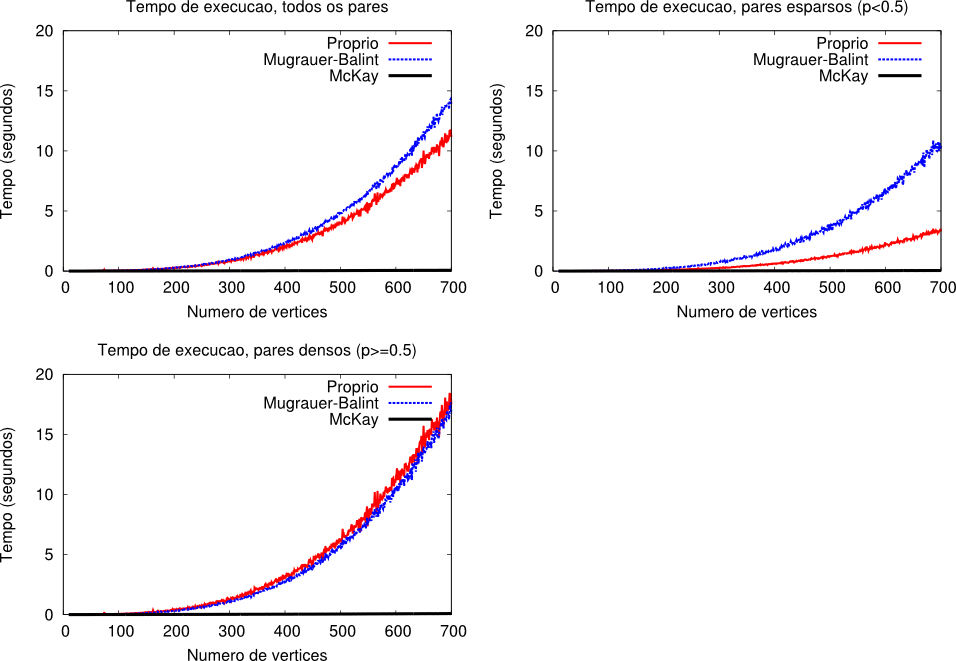
\includegraphics[scale=1.1]{fig1.png} \\

Note que o algoritmo de McKay se mostra muito mais eficiente que qualquer uma das codificações. Isso se deve principalmente, ao 
fato do algoritmo de McKay ser especialmente elaborado para marcações canônicas e testes de isomorfismo, mas também, em parte, ao fato 
dos algoritmos de codificação não serem altamente otimizados e, finalmente, ao uso do minisat, que não é, no momento, o mais eficiente 
SAT-solver disponível.

Note também que, para grafos esparsos, a nossa codificação é significativamente mais eficiente que a de Mugrauer e Balint. Isso se deve 
ao número de cláusulas em nossa codificação ser extremamente baixo para grafos esparsos, e positivamente correlacionado com o número de 
arestas, enquanto o número de cláusulas na codificação de Mugrauer e Balint para grafos esparsos é muito próximo ao número de 
cláusulas para grafos densos. Isso pode ser constatado num nível intuitivo ao se construir uma fórmula na codificação Mugrauer-Balint 
para um grafo de $n$ vértices e apenas uma aresta, e comparar com uma fórmula na mesma codificação para o grafo resultante da remoção 
de uma aresta de $K_n$.

Por outro lado, a codificação de Mugrauer e Balint se mostra ligeiramente mais eficiente no caso de grafos densos. Isso se deve ao fato 
de que, apesar do número de cláusulas em sua codificação geralmente ser, tanto para grafos esparsos quanto densos, maior que o número 
na nossa codificação, as cláusulas de restrição são mais ``dedutivas'', no sentido de que são todas cláusulas binárias, o que implica 
que qualquer literal decidido desencadeia, potencialmente, numerosas propagações unitárias, o que pode levar mais rapidamente a uma 
valoração que satisfaz a fórmula ou a uma contradição. Além disso, a diferença no número de cláusulas entre instâncias reduzidas pelas 
duas codificações torna-se menor quanto mais densos os grafos são.

O gráfico a seguir mostra o tempo médio de execução em função da probabilidade de aresta das instâncias.\\

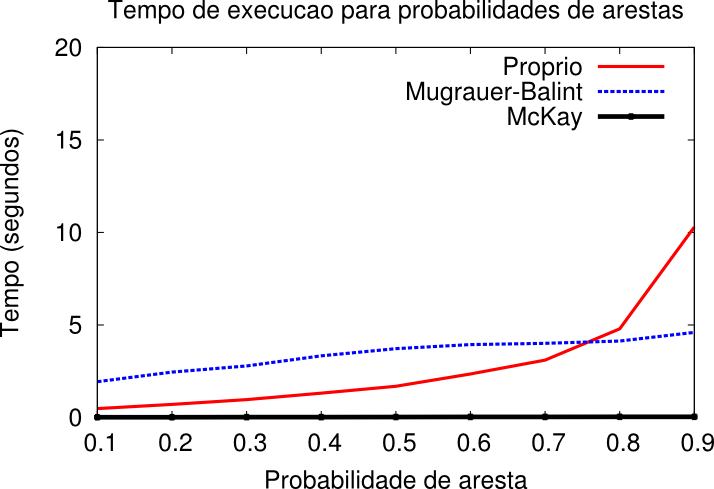
\includegraphics[scale=1.0]{fig2.png}\\

Note que o aumento no tempo de execução com relação à probabilidade de aresta na codificação de Mugrauer e Balint é tênue, enquanto na 
nossa codificação, ele torna-se íngreme ao se chegar nas maiores probabilidades. Observando-se esse fato, uma modificação que pode 
levar a nossa codificação a superar a de Mugrauer e Balint em todas as densidades, baseada no fato de que grafos isomorfos também tem 
complementos isomorfos, é construir cláusulas de restrição baseadas nos complementos dos grafos, no caso de instâncias com um
número muito grande de arestas.

\bibliographystyle{plainnat}
\bibliography{fun_logicos}

\end{document}
